\title{wBox -- Der Lautsprecher f\"ur Ihr Netzwerk}

\team{%
    Yannick Bürgi,
    Nino Feracin,
    David Mettler,
    Franziska Neuhaus,
    Ueli Strebel,
    Marco Wassmer,
    Eric Zimmermann}

\client{Matthias Meier}

\coaches{%
    Matthias Meier,
    Peter Ganzmann,
    Anita Gertiser,
    Ingrid Giel,
    Bonnie Domenghino}

\fssummary{
    Heimkommen  und  mit  einem  Klick  auf das  Handy  die  Musik  anschalten
    und  geniessen. Dies  können  Sie  nun ganz  einfach  mit  unserem  neuen
    Netzwerklautsprecher \emph{wBox}. Spielen  Sie Musik ab,  ohne langwierige
    Kabel und einfach vom Handy zu bedienen.
}

\fsgraphics{
    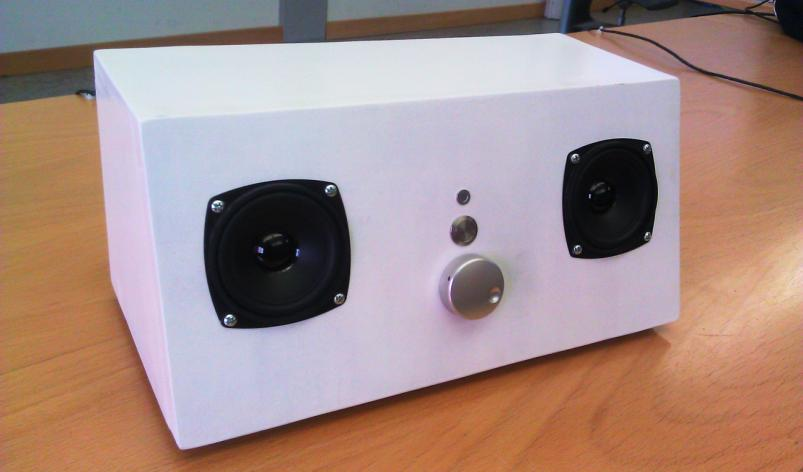
\includegraphics[width=0.64\textwidth,height=55mm]{images/wbox0}
    \hfill
    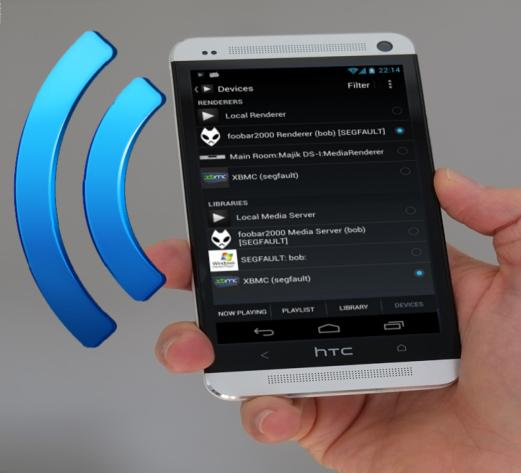
\includegraphics[width=0.34\textwidth,height=55mm]{images/wbox1}
    \graphicscaption{Links: wBox Frontansicht, Rechts: Handy mit Netzwerkzugang}
}

\fscontent{
    \section{Die Aufgabe}
    Immer   mehr  Geräte   können   digitale  Medien   über  das   Netzwerk
    abspielen. Begonnen    hat   dieser    Trend   mit    Apple   und    ihrem
    AirPlay-Protokoll. Dieses  Protokoll ist  zum  Einen teuer  und von  Apple
    zu   zertifizieren.   Deshalb   eine  Vereinigung   von  Herstellern   das
    DLNA-Protokoll erstellt. DLNA eignet sich vor allem für unser Projekt, da
    es auch in  Open-Source Projekten einsetzbar ist.   Da drahtlose Produkte,
    mit einer guten Qualität, auf dem heutigen Markt recht teuer sind, war es
    nun unser Auftrag ein solches netzwerkfähiges Abspielgerät in Form eines
    Musiklautsprechers, zu  ent- wickeln.   Um eine gute  Energieeffizienz und
    kleinere  Grössen zu  erreichen, sollte  ein digitaler  Audio-Verstärker
    verwendet werden.

    \newcol
    \section{Die L\"osung}
    Das Lautsprechergehäuse wurde aus Holz gefertigt. Dies diente einer guten
    Klangqualität. Die  Vorderseite wurde  zudem  schräg konstruiert,  damit
    die Schallwellen  breiter ausgesendet  werden können.   Als Steuereinheit
    beinhaltet die wBox  ein Raspberry Pi, auf dem  alle notwendigen Programme
    laufen und  das die Verbindung zum  Heimnetz herstellt.  Es kann  per DLNA
    mit mehreren Geräten gleichzeitig auf die wBox zugegriffen werden.

    \newcol
    \section{Die Handhabung}
    Zur   einfachen  Bedienung   wurden  auf   der  Vorderseite   sehr  wenige
    Bedienelemente angebracht,  um das  Gerät mit  einem lokalen  Netzwerk zu
    verbinden sowie die Lautstärke  zu regeln. Eine Status-LED vermittelt dem
    Benutzer zusätzlich  mit verschiedenen  Farben den momentanen  Status des
    Laut-  sprechers.  Die  wBox  kann mit  einem  einfachen Tastendruck  eine
    Verbindung zu Ihrem WLAN-Netzwerk aufbauen.   Da sie lediglich eine Strom-
    versorgung  benötigt,  kann  sie  praktisch an  jedem  Standort  platzier
    werden.
}

\infobox{\textbf{D}igital \textbf{L}iving \textbf{N}etwork \textbf{A}lliance}{%
    Stellt    eine   Vereinigung    von    Herstellern    von   Computern    ,
    Unterhaltungselektronik  und  Mobiltelefonen  dar,  um  die  Kommunikation
    zwischen den Geräten der verschiedenen Hersteller sicherzustellen.

    Zu den  Hauptaufgaben der Organisation gehört  die gemeinsame Entwicklung
    und laufende Aktualisierung technischer Leitlinien

    Mithilfe  des DLNA-Protokoll  können die  verschiedensten Heimnetzgeräte
    miteinander  kommunizieren. Es   stellt  auch  eine  alternative   zu  dem
    lizenzpflichtigen AirPlay von Apple dar.
}
